\subsection{Интегрирование дифференциальных форм на дифференцируемых многообразиях}

Некоторые определения этого параграфа составлены автором на основе курса дифференциальной геометрии и топологии из третьего семестра и отличаются от лекционных (но различия в рамках данного параграфа несущественны).

\begin{designation}
Условимся в этом параграфе писать индексы в круглых скобках, а аргументы функции в квадратных, например $\phi(i)[u]$.
\end{designation}

\begin{definition}
	Клетки $M(i)$ и $M(j)$ класса $C^k$ называются \textit{сцепленными}, если выполнены условия:
	\begin{enumerate}
		\item $M(i,j) := M(i) \cap M(j) \neq \emptyset$,
		
		\item Отображение $\pi(i, j) := \psi(i) \circ \phi(j) \colon \psi(j)[M(i,j)] \to \psi(i)[M(i,j)]$ является диффеоморфизмом класса $C^k$.
	\end{enumerate}
	При этом $\pi(i,j)$ называется \textit{сцепляющим диффеоморфизмом}.
\end{definition}

\begin{designation}
Будем также обозначать $K(i,j) := \psi(i)[M(i,j)]$, $K(j,i) := \psi(j)[M(i,j)]$ (порядок индексов важен).
\end{designation}

\begin{center}
	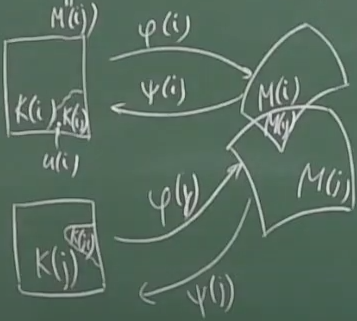
\includegraphics[width=0.4\textwidth]{images/manifold.png}
\end{center}

\begin{definition} (изменено автором)
	Подмножество $\R^n$ называется \textit{$m$-мерным дифференцируемым (гладким) многообразием класса $C^k$}, если оно является не более чем счётным объединением клеток $\{M(i)\}_{i \in \mathcal I}$ класса $C^k$ таких, что любые две пересекающиеся клетки сцеплены.
\end{definition}

\begin{definition} (изменено автором)
	Зафиксируем конкретный набор клеток $\{M(i)\}_{i \in \mathcal I}$ в определении многообразия $M$ и для каждой клетки $M(i)$ возьмём конкретную параметризацию.
	Тогда клетка $M(i)$ многообразия $M$ вместе со своим координатным отображением $\psi(i)$ называется \textit{картой}. Набор карт $\{(M(i), \psi(i))\}_{i \in \mathcal I}$ называется \textit{атласом многообразия M}.
\end{definition}

\begin{anote}
	В нашем представлении гладкое многообразие --- это некое "хорошее" \ подмножество $\R^n$, поддающееся гладкой параметризации. Но вообще говоря многие другие топологические пространства можно рассматривать как гладкие многоообразия. Отличие от $\R^n$ лишь в том, что в общем случае нельзя определить понятие дифференцируемости параметризующего отображения, но непрерывность остаётся. При этом сцепляющий диффеоморфизм всё ещё должен быть диффеоморфизмом. Если же считать, что мы работаем с $\R^n$ и $\phi$ само по себе диффеоморфизм, то из леммы \ref{main_diffeomorphism_lemma} следует, что требование к $\pi(i,j)$ быть диффеоморфизмом эквивалентно тому, что прообразы пересечения клеток открыты в $\R^m$.
\end{anote}

\begin{example}
	Трёхмерная сфера $\{x^2 + y^2 + z^2 = 1\}$ может быть параметризована, например, двумя кубами $\{-3 < x, y < 3, z = \pm1\}$ с помощью стереографической проекции. В качестве упражнения можно убедиться, что такая параметризация будет гладкой.
	\begin{center}
		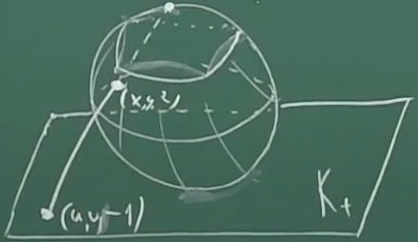
\includegraphics[width=0.4\textwidth]{images/sphere_manifold.png}
	\end{center}
\end{example}

\begin{example}
	Если $M_1 = \bigcup_{i \in \mathcal I} M_1(i)$, $M_2 = \bigcup_{j \in \mathcal J} M_2(j)$ --- $m$- и $n$-мерные многообразия, то $M_1 \times M_2 = \bigcup_{i \in \mathcal I} \bigcup_{j \in \mathcal J} M_1(i) \times M_2(j)$ --- $(m+n)$-мерное многообразие. Параметризацию определим естественным образом:
	\[
		\ps{\phi_1(i) \times \phi_2(j)}[x, y] = \phi_1(i)[x] \times \phi_2(j)[y]
	\]
	Ранг её матрицы Якоби равен сумме рангов $\phi_1(i)$ и $\phi_2(j)$ и потому максимален:
	\[
		 (\phi_1(i) \times \phi_2(j))' =
		 \Matrix{
			&{\phi_1'(i)}& &{0}
			\\
			&{0}& &{\phi_2'(j)}
		}
	\]
\end{example}

\begin{note}
	Далее считаем все многообразия связными, а атласы конечными.
\end{note}

\begin{definition} (от автора)
	Функция $f$, заданная на многообразии $M$ с атласом $\{(M(i), \psi(i))\}_{i=1}^N$, называется \textit{$C^k$-гладкой}, если для любой клетки $M(i)$ композиция $f \circ \phi(i)$ является $C^k$-гладкой.
\end{definition}

\begin{definition}
	\textit{Разбиением единицы, подчинённым атласу $\{(M(i), \psi(i))\}_{i=1}^N$}, называется набор функций $\{\zeta(i) \colon M \to \R\}_{i=1}^N$, обладающих следующими свойствами:
	\begin{enumerate}
		\item
		$\zeta(i)$ имеют ту же гладкость, что и $M$.
		\item
		$\forall x \in M \ \zeta(i)[x] \geq 0$, причём $\zeta(i)[x] > 0 \Lra x \in M(i)$
		\item
		$\forall x \in M \ \sum_{i=1}^N \zeta(i)[x] = 1$
	\end{enumerate}
\end{definition}

\begin{theorem}
	На любом гладком многообразии $M$ существует разбиение единицы, подчинённое атласу $\{(M(i), \psi(i))\}_{i=1}^N$.
\end{theorem}

\begin{proof}
	Определим на параметризующем кубе $K$ такую функцию:
	\[
		\widehat{\eta(i)}[u] := \prod_{s=1}^m \exp\ps{-\frac{1}{(u^s)^2 (1-u^s)^2}}
	\]
	Можно проверить, что это $C^\infty$-гладкая функция, причём положительная в любой точке $K$, и все её производные стремятся к нулю при приближении к границе $K$. На самом многообразии же определим
	\[
		\eta(i)[x] := \System{
		&{\widehat{\eta(i)}[\psi(i)[x]], \ x \in M(i)}
		\\
		&{0, \ x \notin M(i)}}
	\]
	Так как любая точка многообразия принадлежит некоторой клетке $M(i)$, для которой $\eta(i)(x) > 0$, искомое разбиение единицы можно сделать таким:
	\[
		\zeta(i)[x] := \frac {\eta(i)[x]} {\sum\limits_{j=1}^N \eta(j)[x]}
	\]
	Проверим, что это гладкая функция. Из определения гладкости на многообразии понятно, что достаточно проверить гладкость $\eta(i)$. Сделаем это:
	\[
		\eta(i)[\phi(j)[u]] = \System{
		&{ \widehat{\eta(i)}[\pi(i,j)[u]], \ \phi(j)[u] \in M(i)}
		\\
		&{0, \ \phi(j)[u] \notin M(i)}}
	\]
	При этом $\phi(j)[u] \in M(i) \Lolra u \in K(j,i)$. Как мы помним, на $K(j,i)$ $\pi(i,j)$ является диффеоморфизмом и проблем не возникает, как и на дополнении к его замыканию. На границе же предлагается поверить, что $\pi(i,j)[u] \to \partial K$ при $u \to \partial K(j,i) \setminus \partial K$, а потому $\widehat{\eta(i)}^{(k)}[\pi(i,j)[u]] \to 0$. Из этого следует, что $\eta(i)$ имеет ту же гладкость, что и $\pi(i,j)$, а вместе с тем и $\zeta(i)$.	Остальные свойства разбиения единицы, очевидно, выполняются: $\zeta(i)[x] = 0 \Lra \eta(i)[x] = 0 \Lra x \notin M(i)$ и $\sum_{i=1}^N \zeta(i) = 1$.
\end{proof}

\begin{note}
	Так же, как и в случае с клетками, определяется \textit{касательное пространство} в каждой точке многообразия и \textit{касательное расслоение} $(x, T(x))$. По лемме \ref{tangent_space_vs_param} касательное пространство не зависит ни от клетки, покрывающей точку, ни от атласа. Аналогично определяются и дифференциальные формы на многообразии.
\end{note}

\begin{definition} (от автора)
	\textit{Дифференциалом} $p$-формы $\Omega$, заданной на многообразии $M$, называется форма
	\[
		d\Omega := \sum_{i=1}^N  d\ps{\zeta(i) \Omega\big|_{M(i)}}
	\]
\end{definition}

\begin{definition}
	Если $\Omega$ --- дифференциальная форма, заданная на многообразии M, то \textit{интеграл от $\Omega$ по M} можно определить как
	\[
		\int_M \Omega \ := \ \sum_{i=1}^N \int_{M_i} \zeta(i)\Omega
	\]
\end{definition}

\begin{note}
	Разумеется, в определениях выше нужно доказывать независимость от атласа и от разбиения единицы. Мы же примем этот факт на веру. Однако линейность интеграла по многообразию сразу следует из линейности интеграла по клетке --- это нам пригодится.
\end{note}

\begin{definition}
	Многообразие называется \textit{ориентируемым}, если на всех его клетках можно задать ориентацию согласованно, то есть для любой точки $x \in M(i) \cap M(j)$ выбранные положительные базисы в $T_{M(i)}(x)$ и $T_{M(j)}(x)$ ориентированы согласованно.
\end{definition}

\begin{example}
	Стандартный пример неориентируемого многообразия --- лента Мёбиуса. Неформально неориентируемость здесь объясняется тем, что внешняя нормаль к клетке обязательно перейдёт во внутреннюю, сделав один круг вдоль ленты.
\end{example}

\begin{proposition}
	Многообразие M ориентируемо в том и только том случае, когда на нём существует непрерывная невырожденная дифференциальная форма старшей валентности (порядка). При этом, если последнее выполняется, то ориентация задаётся значением этой формы на базисах соответствующих касательных пространств.
\end{proposition}

\begin{proof}
	Докажем лишь необходимость. Если M --- элементарное многообразие, то для него форма ориентированного объёма удовлетворяет требованиям. Пусть теперь есть сцепленные клетки $M(i)$ и $M(j)$ с формами ориентированного объёма $V(i)$ и $V(j)$ соответственно. Поскольку валентность этих форм максимальна, они отличаются друг от друга умножением на некоторый коэффициент:
	\[
		V(i)[x] = \alpha(i, j)V[j][x],
	\]
	причём $\alpha(i, j) > 0$ в силу согласованности ориентации на $M(i)$ и $M(j)$. С учётом этого определим общую дифформу $V$:
	\[
		V[x] := \sum_{i=1}^N \zeta(i)[x] V(i)[x],
	\]
	которая непрерывна и невырождена из тех же свойств $V(j)$, поскольку имеет место такое её представление:
	\[
		\forall x \in M(j) \ \ V[x] = \ps{\sum_{M(i) \cap M(j) \neq \emptyset} \zeta(i)[x] \, \alpha(i, j)} V(j)[x]
	\]
\end{proof}

\begin{definition}
	Для ориентируемого многообразия \textit{форма ориентированного объёма} задаётся как
	\[
		V[x] := \sum_{i=1}^N \zeta(i)[x] V_{M(i)}[x]
	\]
\end{definition}

\begin{note}
	Снова опускаем проверку корректности определения.
\end{note}

\begin{definition}
	Многообразие M называется \textit{замкнутым}, если оно является замкнутым множеством в $\R^n$.
\end{definition}

До этого момента все параметризующие кубы у нас были открыты (что, однако, не мешает многообразию быть замкнутым). Теперь, чтобы подобраться к теореме Стокса-Пуанкаре, нам предстоит разобраться с границей многообразия.

\begin{definition}
	Клетка $M(i)$ называется \textit{сингулярной клеткой многообразия $M$}, если некоторая её грань $M_\alpha^s(i) \not\subset M$. В противном случае клетка называется \textit{регулярной}.
\end{definition}

\begin{center}
	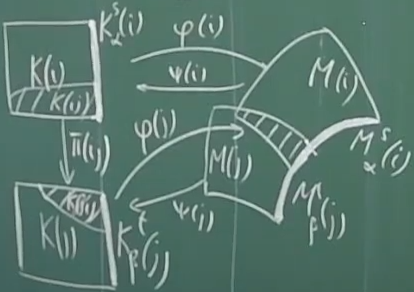
\includegraphics[width=0.4\textwidth]{images/manifold_border.png}
\end{center}

\begin{note}
	Далее ограничимся атласами, в которых у каждой клетки не более одной грани обладает этим свойством (но для удобства обозначений будем считать, что ровно одна), причём $M_\alpha^s(i) \cap M = \emptyset$, а \textit{край многообразия} $\partial M := \bigcup_{i=1}^N M_\alpha^s(i)$ образует связное множество.
\end{note}

\begin{note}
	Грань $M_\alpha^s(i)$ отдельно взятой $m$-мерной клетки сама является $(m-1)$-мерной клеткой с параметризацией, индуцированной $\phi(i)$. Если наложить на пересекающиеся грани условие сцепленности, то край многообразия тоже будет многообразием размерности на 1 меньше. Более того, можно показать, что край ориентируемого многообразия ориентируем.
\end{note}

\begin{designation}
	Введём естественные обозначения для клетки с границей $M_\alpha^s(i)$ и всего многообразия с краем:
	\[
		\ole{M}(i) := M(i) \cup M_\alpha^s(i)
	\]
	\[
		\ole{M} := M \cup \partial M
	\]
\end{designation}

\begin{anote}
	Край многообразия не следует путать с топологической границей. Действительно, если $n > m$, то, как известно, мера образа параметризующего куба равна нулю, а значит, у него не будет внутренности и все точки будут граничными.
\end{anote}

\begin{lemma}
	Пусть $\{(M(i), \psi(i))\}_{i=1}^N$ --- атлас многообразия M гладкости $C^k$, \\ $\{(M_\alpha^s(i), \psi_\alpha^s(i))\}_{i=1}^N$ --- атлас многообразия $\partial M$. Тогда существует разбиение единицы, подчинённое этим атласам, т.е.
	\begin{enumerate}
		\item
		$\zeta(i) \in C^k$ на $\ole M$
		\item
		$\forall x \in \ole M \ \zeta(i)[x] \geq 0$ и $\zeta(i)[x] > 0 \Lra x \in \ole{M}(i)$
		\item
		$\forall x \in \ole M \ \sum_{i=1}^N \zeta(i)[x] = 1$
	\end{enumerate}
\end{lemma}

\begin{proof}
	"Подкрутим" \ уже построенное разбиение таким образом, чтобы нужная координата куба могла обращаться в 0 или 1:
	\begin{gather*}
		f(t) := \System{
			&\exp\ps{-\frac{1}{t^2(1-t)^2}}, \ t \in (0, 1) \\
			&0, \ t \in \{0, 1\}
		}
		\\
		\widehat{\eta(i)}[u] := \System{
			\int_0^{u^{s(i)}} \! f(t)dt \, \prod_{r \neq s(i)} f(u^r), \ \alpha(i) = 1
			\\
			\int_{u^{s(i)}}^1 \! f(t)dt \, \prod_{r \neq s(i)} f(u^r), \ \alpha(i) = 0}
		\\
		\eta(i)[x] := \System{
			&{\widehat{\eta(i)}[\psi(i)[x]], \ x \in \ole{M}(i)}
			\\
			&{0, \ x \notin \ole{M}(i)}}
		\\
		\zeta(i)[x] := \frac {\eta(i)[x]} {\sum\limits_{j=1}^N \eta(j)[x]}
	\end{gather*}
	$\eta(i)$ определены на $\ole{M}(i)$ и имеют гладкость $C^k$ по тем же причинам, что и раньше. Детали опускаются, однако мы пользуемся тем, что сингулярная грань не пересекается с многообразием, иначе $\zeta(i)$ не была бы дифференцируема (даже в одностороннем смысле) на этой грани.
\end{proof}

\begin{note}
	Далее $\zeta(i)$ означает разбиение единицы для многообразия с краем. При этом по нашему соглашению на край оно же годится для того же многообразия без края.
\end{note}

\begin{theorem} (Стокса-Пуанкаре для дифференцируемого многообразия с краем)
	Пусть $\Omega$ --- дифференциальная $(m-1)$-форма, заданная на ориентируемом многообразии $M$ с краем $\partial M$. Тогда
	\[
		\int_{\partial M} \Omega = \int_{M} d\Omega,
	\]
	где
	\[
		\int_{\partial M} \Omega = \sum_{i=1}^N \int_{\partial M(i)} \zeta(i) \Omega
	\]
\end{theorem}

\begin{proof}
	Воспользуемся линейностью, свойствами разбиения единицы и уже доказанной версией теоремы для клетки:
	\[
		\int_{M} d\Omega = \sum_{i=1}^N \int_{M} d(\zeta(i) \Omega) = \sum_{i=1}^N \int_{M(i)} d\ps{\zeta(i) \Omega} = \sum_{i=1}^N \int_{\partial M(i)} \zeta(i) \Omega = \int_{\partial M} \Omega
	\]
\end{proof}

\begin{anote}
	Формально в этом доказательстве есть две проблемы.
	\begin{enumerate}
		\item Второй переход вовсе не очевиден. По определению нам нужно показать следующее равенство:
		\[
			\sum_{i=1}^N \sum_{j=1}^N \int_{M(j)} \zeta(j) d(\zeta(i) \Omega) = \sum_{i=1}^N \int_{M(i)} d\ps{\zeta(i) \Omega}
		\]
		Что сводится к проверке равенства каждой пары слагаемых по отдельности:
		\[
			\sum_{j=1}^N \int_{M(j)} \zeta(j) d(\zeta(i) \Omega) = \int_{M(i)} d\ps{\zeta(i) \Omega}
		\]
		$\zeta(i)\Omega$ тождественно равна нулю во всех клетках, не пересекающихся с $M(i)$, и легко проверить, что дифференцирование сохраняет это свойство. Однако отсюда всё ещё напрямую не следует равенство. Обозначим $\Pi := d(\zeta(i)\Omega)$ и распишем левую часть:
		\[
			\sum_{j=1}^N \int_{M(j)} \zeta(j) \Pi = \sum_{j=1}^N \int_{K} \phi(j)^*(\zeta(j) \Pi)
		\]
		Подынтегральная форма обнуляется везде, кроме, быть может, пересечения клеток $M(i)$ и $M(j)$. То есть мы знаем, по какому участку куба идёт интегрирование:
		\[
			\sum_{j=1}^N \int_{K} \phi(j)^*(\zeta(j) \Pi) = \sum_{j=1}^N \int_{K(j,i)} \phi(j)^*(\zeta(j) \Pi)
		\]
		Теперь можно сделать перенос формы с помощью $\pi(j,i)^*$. И хотя мы это явно не оговаривали, можно считать, что знак интеграла не поменяется в силу ориентируемости многообразия (и именно здесь мы ей пользуемся!) и положительности параметризации:
		\[
			\sum_{j=1}^N \int_{K(j,i)} \phi(j)^*(\zeta(j) \Pi) = \sum_{j=1}^N \int_{K(i,j)} (\pi(j,i)^* \circ \phi(j)^*)(\zeta(j) \Pi) = \sum_{j=1}^N \int_{K(i,j)} \phi(i)^*(\zeta(j) \Pi)
		\]
		Теперь снова вспомним, что последняя форма зануляется вне $K(i,j)$, и поэтому можно интегрировать по всему кубу:
		\[
			\sum_{j=1}^N \int_{K(i,j)} \phi(i)^*(\zeta(j) \Pi) = \sum_{j=1}^N \int_{K} \phi(i)^*(\zeta(j) \Pi)
		\]
		Наконец, понятно, что и интеграл по кубу, и перенос формы фиксированы и линейны, что завершает длинную цепочку равенств:
		\[
			\sum_{j=1}^N \int_{K} \phi(i)^*(\zeta(j) \Pi) = \int_{K} \phi(i)^*\ps{\sum_{j=1}^N \zeta(j) \Pi} = \int_{K} \phi(i)^*\Pi = \int_{M(i)} \Pi
		\]
		\item
		Мы доказывали теорему Стокса-Пуанкаре для куба и для клетки в предположении, что форма определена и гладка в некоторой их окрестности, чего не скажешь про $\zeta(i)\Omega$. Здесь есть два пути. Первый --- научиться дифференцировать форму на границе куба/клетки, даже если её нельзя продолжить. Это в принципе несложно: нужно просто брать одностороннюю частную производную по переменной, соответствующей грани куба. Однако про это нужно явно сказать, поскольку изначально мы определяли дифференциальные формы именно в области. Второй способ --- гладко продлить функции $\zeta(i)$ за счёт того, что диффеоморфизмы $\phi(i)$ у нас по-прежнему определены на чуть большем кубе $K_\eps \supset K$. Я представляю, как можно было бы доопределить $\zeta(i)$ до $M_\eps(i)$ так, чтобы они не изменились на $\ole M(i)$, но формулы получатся ещё сложнее (это не то же самое, что завести разбиение единицы на атласе с клетками $M_\eps(i)$). В любом случае, эта деталь нуждается в уточнении.
	\end{enumerate}
\end{anote}